\documentclass{article}


\usepackage{arxiv}

\usepackage[utf8]{inputenc} % allow utf-8 input
\usepackage[T1]{fontenc}    % use 8-bit T1 fonts
\usepackage{hyperref}       % hyperlinks
\usepackage{url}            % simple URL typesetting
\usepackage{booktabs}       % professional-quality tables
\usepackage{amsfonts}       % blackboard math symbols
\usepackage{nicefrac}       % compact symbols for 1/2, etc.
\usepackage{microtype}      % microtypography
\usepackage{lipsum}
\usepackage{graphicx}


\newcommand{\argmin}{\arg\!\min}
%\newcommand{\st}{\mathrm{s.\,t.}}
\newcommand{\Amat}{{\boldsymbol A}}
\newcommand{\Bmat}{{\boldsymbol B}}
\newcommand{\Cmat}{{\boldsymbol C}}
\newcommand{\Dmat}{{\boldsymbol D}}
\newcommand{\Emat}[0]{{{\boldsymbol E}}}
\newcommand{\Fmat}[0]{{{\boldsymbol F}}}
\newcommand{\Gmat}[0]{{{\boldsymbol G}}}
\newcommand{\Hmat}[0]{{{\boldsymbol H}}}
\newcommand{\Imat}{{\boldsymbol I}}
\newcommand{\Jmat}[0]{{{\boldsymbol J}}}
\newcommand{\Kmat}[0]{{{\boldsymbol K}}}
\newcommand{\Lmat}[0]{{{\boldsymbol L}}}
\newcommand{\Mmat}[0]{{{\boldsymbol M}}}
\newcommand{\Nmat}[0]{{{\boldsymbol N}}}
\newcommand{\Omat}[0]{{{\boldsymbol O}}}
\newcommand{\Pmat}[0]{{{\boldsymbol P}}}
\newcommand{\Qmat}[0]{{{\boldsymbol Q}}}
\newcommand{\Rmat}[0]{{{\boldsymbol R}}}
\newcommand{\Smat}[0]{{{\boldsymbol S}}}
\newcommand{\Tmat}[0]{{{\boldsymbol T}}}
\newcommand{\Umat}{{{\boldsymbol U}}}
\newcommand{\Vmat}[0]{{{\boldsymbol V}}}
\newcommand{\Wmat}[0]{{{\boldsymbol W}}}
\newcommand{\Xmat}{{\boldsymbol X}}
\newcommand{\Ymat}[0]{{{\boldsymbol Y}}}
\newcommand{\Zmat}{{\boldsymbol Z}}

\newcommand{\av}{\boldsymbol{a}}
\newcommand{\Av}{\boldsymbol{A}}
\newcommand{\Cv}{\boldsymbol{C}}
\newcommand{\bv}{\boldsymbol{b}}
\newcommand{\cv}{{\boldsymbol{c}}}
\newcommand{\dv}{\boldsymbol{d}}
\newcommand{\ev}[0]{{\boldsymbol{e}}}
\newcommand{\fv}{\boldsymbol{f}}
\newcommand{\Fv}[0]{{\boldsymbol{F}}}
\newcommand{\gv}[0]{{\boldsymbol{g}}}
\newcommand{\hv}[0]{{\boldsymbol{h}}}
\newcommand{\iv}[0]{{\boldsymbol{i}}}
\newcommand{\jv}[0]{{\boldsymbol{j}}}
\newcommand{\kv}[0]{{\boldsymbol{k}}}
\newcommand{\lv}[0]{{\boldsymbol{l}}}
\newcommand{\mv}[0]{{\boldsymbol{m}}}
\newcommand{\nv}{\boldsymbol{n}}
\newcommand{\ov}[0]{{\boldsymbol{o}}}
\newcommand{\pv}[0]{{\boldsymbol{p}}}
\newcommand{\qv}[0]{{\boldsymbol{q}}}
\newcommand{\rv}[0]{{\boldsymbol{r}}}
\newcommand{\sv}[0]{{\boldsymbol{s}}}
\newcommand{\tv}[0]{{\boldsymbol{t}}}
\newcommand{\uv}[0]{{\boldsymbol{u}}}
\newcommand{\vv}{\boldsymbol{v}}
\newcommand{\wv}{\boldsymbol{w}}
\newcommand{\Wv}{\boldsymbol{W}}
\newcommand{\xv}{\boldsymbol{x}}
\newcommand{\yv}{\boldsymbol{y}}
\newcommand{\Xv}{\boldsymbol{X}}
\newcommand{\Yv}{\boldsymbol{Y}}
\newcommand{\zv}{\boldsymbol{z}}

\newcommand{\xvf}{\widetilde{\xv}}
\newcommand{\Fmb}{\boldsymbol{\mathcal{F}}}

\newcommand{\Gammamat}[0]{{\boldsymbol{\Gamma}}}
\newcommand{\Deltamat}[0]{{\boldsymbol{\Delta}}}
\newcommand{\Thetamat}{\boldsymbol{\Theta}}
\newcommand{\Lambdamat}{{\boldsymbol{\Lambda}}}
\newcommand{\Ximat}[0]{{\boldsymbol{\Xi}}}
\newcommand{\Pimat}[0]{{\boldsymbol{\Pi}} }
\newcommand{\Sigmamat}{\boldsymbol{\Sigma}}
\newcommand{\Upsilonmat}[0]{{\boldsymbol{\Upsilon}} }
\newcommand{\Phimat}{\boldsymbol{\Phi}}
\newcommand{\Psimat}{\boldsymbol{\Psi}}
\newcommand{\Omegamat}{{\boldsymbol{\Omega}}}

\newcommand{\Lambdav}{\bm{\Lambda}}
\newcommand{\alphav}{\boldsymbol{\alpha}}
\newcommand{\betav}[0]{{\boldsymbol{\beta}} }
\newcommand{\gammav}{{\boldsymbol{\gamma}}}
\newcommand{\deltav}[0]{{\boldsymbol{\delta}} }
\newcommand{\epsilonv}{\boldsymbol{\epsilon}}
\newcommand{\zetav}[0]{{\boldsymbol{\zeta}} }
\newcommand{\etav}[0]{{\boldsymbol{\eta}} }
\newcommand{\thetav}{\boldsymbol{\theta}}
\newcommand{\iotav}[0]{{\boldsymbol{\iota}} }
\newcommand{\kappav}{{\boldsymbol{\kappa}}}
\newcommand{\lambdav}[0]{{\boldsymbol{\lambda}} }
\newcommand{\muv}{\boldsymbol{\mu}}
\newcommand{\nuv}{{\boldsymbol{\nu}}}
\newcommand{\xiv}{{\boldsymbol{\xi}}}
\newcommand{\omicronv}[0]{{\boldsymbol{\omicron}} }
\newcommand{\piv}{\boldsymbol{\pi}}
\newcommand{\rhov}[0]{{\boldsymbol{\rho}} }
\newcommand{\sigmav}[0]{{\boldsymbol{\sigma}} }
\newcommand{\tauv}[0]{{\boldsymbol{\tau}} }
\newcommand{\upsilonv}[0]{{\boldsymbol{\upsilon}} }
\newcommand{\phiv}{\boldsymbol{\phi}}
\newcommand{\chiv}[0]{{\boldsymbol{\chi}} }
\newcommand{\psiv}{\boldsymbol{\psi}}
\newcommand{\omegav}[0]{{\boldsymbol{\omega}} }

\newcommand{\tsp}{^{\mathsf{T}}}
\newcommand{\inv}{^{-1}}
\newcommand{\ie}{{\em i.e.}}
\newcommand{\eg}{{\em e.g.}}
\newcommand{\wrt}{{\em w.r.t.\,}}


\title{Dimensionality Reduction}


\author{
  Haoqi~Zhang\\
  \And
  Kaiqi~Jin\\
  \And
  Peihao~Yang\\
  \texttt{516021910233} \\
  \And
  Yi~Zhang\\
}
  
\begin{document}
\maketitle

\begin{abstract}
In this report, we first use support vector machine (SVM) to classify 37322 images with 2048 pre-extracted deep learning features for each image. The data is from the Attributes (AwA2) dataset~\cite{AwA2}. We then reduce the dimensionality in different way and make classification with SVM again. The experiments show that some dimensionality reuction methods are efficient and reliable.
\end{abstract}


% keywords can be removed
\keywords{Dimensionality reduction \and Feature selection \and Feature projection \and Feature learning}


\section{Introduction}
Since the information revolution last century, more and more data has been generated. The dimension curse gradually becomes a critical problem in data science. The last decades have seen plenty of methods to reduce the dimensionality of the data. In this report, we will divide them into three classes, and discuss them based on solid experiment results.

Support vector machine (SVM) is a classical method often applied in the classification tasks~\cite{SVM}. By introducing the kernel trick,  

The Section~\ref{sec:baseline} is the leadin. We will introduce the assessment baseline and assessment criterions applied. The dimensionality reduction methods would be covered in the next three section. In Section~\ref{sec:selection}, we introduce the feature selection methods in detail. We analysis the feature projection methods in Section~\ref{sec:projection}. The feature learning methods are discussed in Section~\ref{sec:learning}. The experiment results and comparisons are in the Section~\ref{sec:discussion}.  In the end, a thorough conclusion is made.


\section{Baseline}
\label{sec:baseline}

\section{Feature selection}
\label{sec:selection}
Feature selection is a kind of methods that directly select some features from the original data. The core of these methods are often the selection criterion. The thought of feature selection is simple but they are efficient and reliable.
\subsection{Theory}
We will introduce the feature selection methods used in our experiments.
\subsubsection{Univariable feature}
This is a forward selection method.

\subsection{Experiment}
This part is mainly about the implementation details and parameter settings. The figure of final results are shown in the Section~\ref{sec:discussion}.

\section{Feature projection}
\label{sec:projection}

\section{Feature learning}
\label{sec:learning}

\section{Discussion}
\label{sec:discussion}
\subsection{SVM parameter setting}
Though in the end, we choose the asked linear SVM to do the comparison experiments for dimensionality reduction, we still make experiment on the SVM parameter setting. The experiment results are shown in the Figure~(\ref{fig:SVM}).

\begin{figure}
	\label{fig:SVM}
	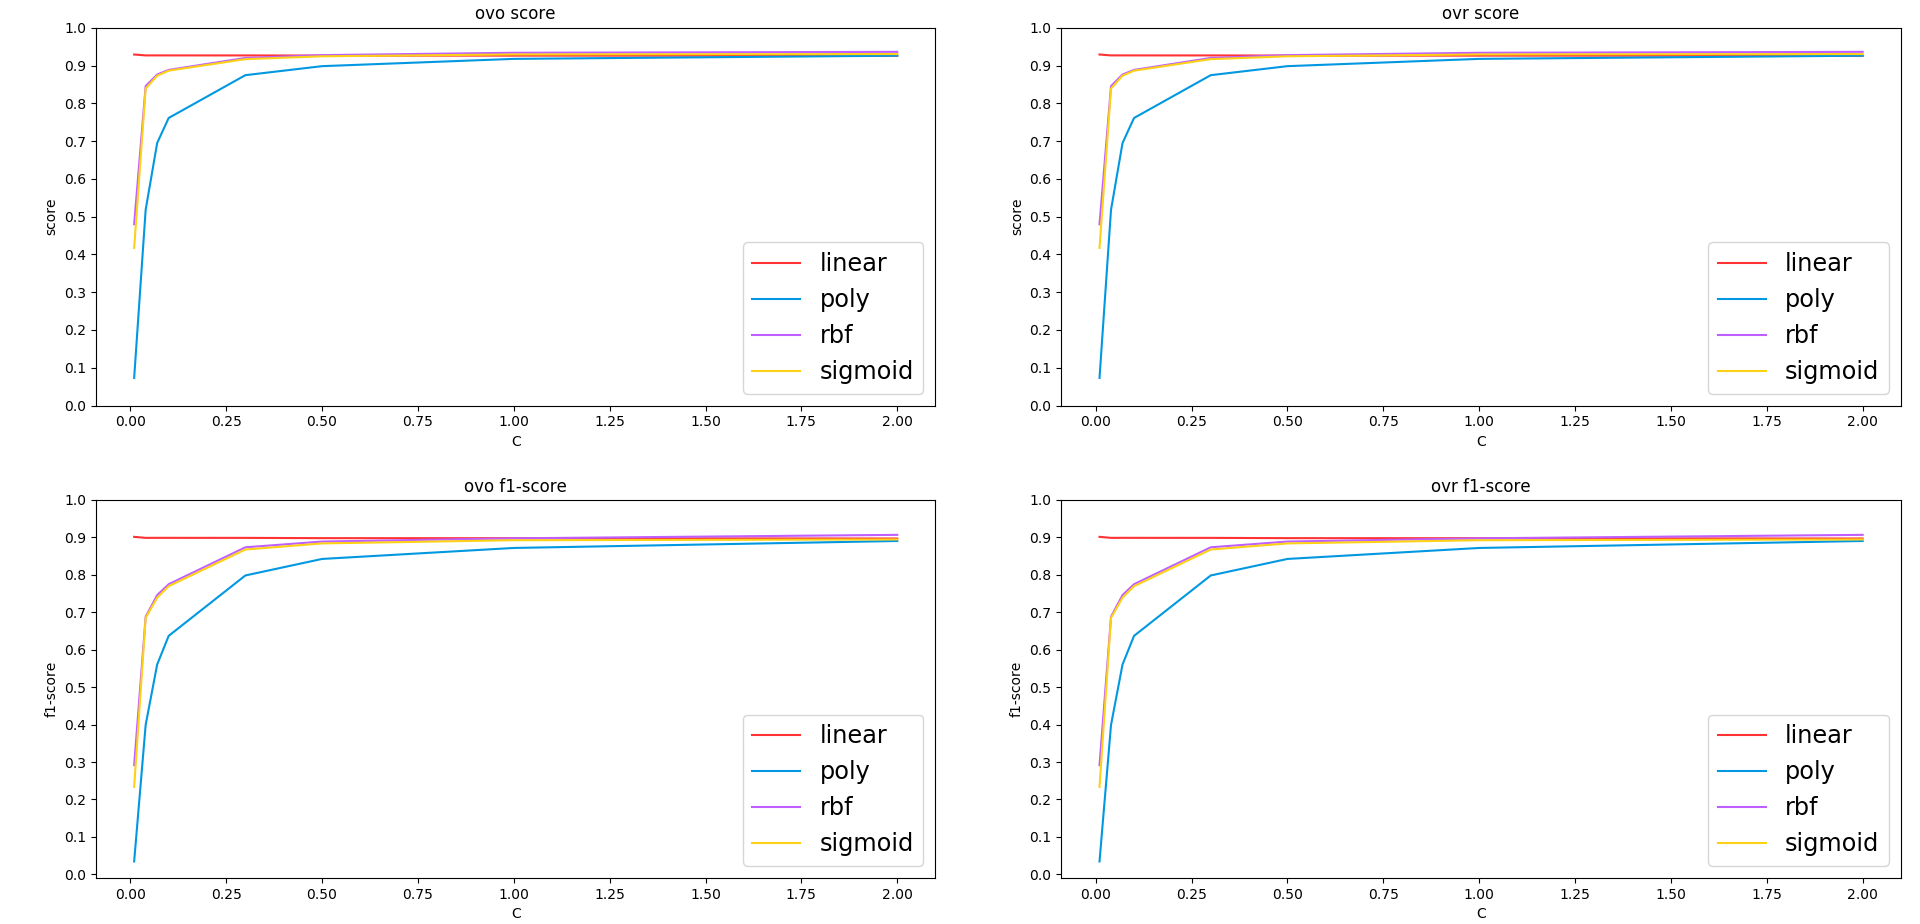
\includegraphics[width=\linewidth]{figs/compare.png}
\end{figure}


\subsection{Reduction on the complete dataset}
Most dimensionality reduction experiments were carried on the complete AwA2 dataset. We changed the number of selected features or other parameters to control the degree of the reduction, and then train linear SVMs on these reduction results. The criterions for the SVM predictions, as mentioned before, are the f1-score and mean accuracy. The comparison is shown in Figure~(\ref{fig:complete}).
  \begin{figure}
  	\label{fig:complete}
  	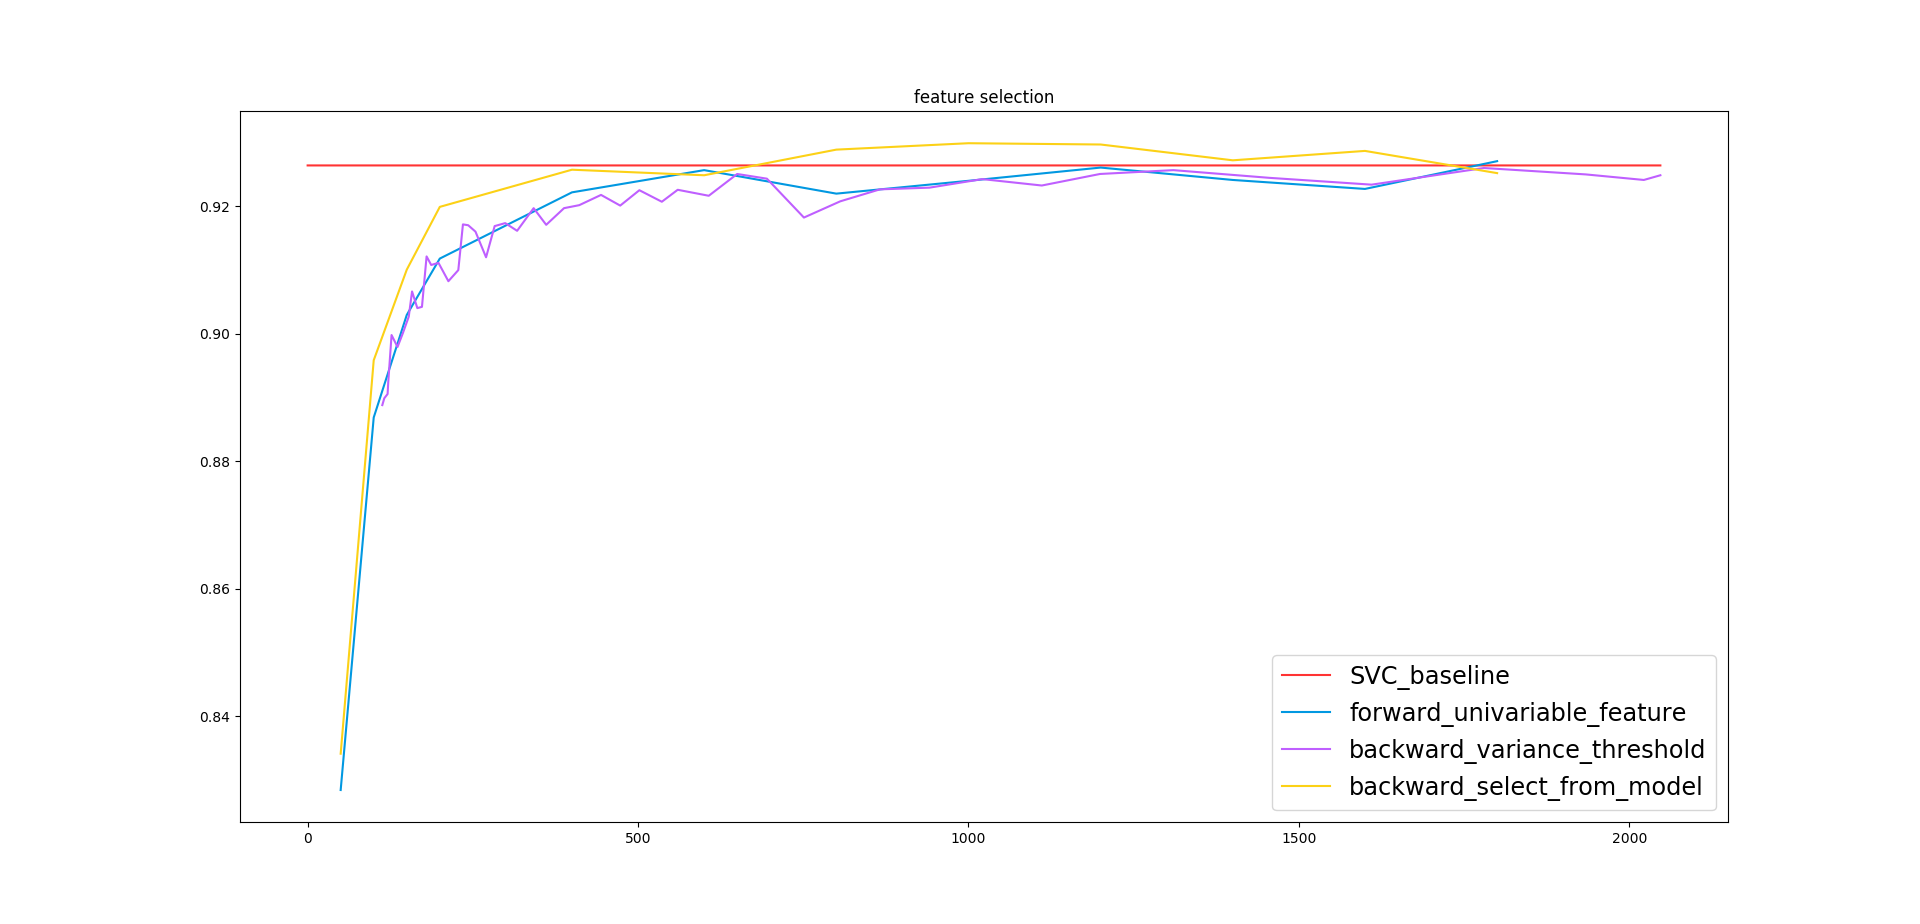
\includegraphics[width=\linewidth]{figs/feature_selection.png}
  \end{figure}

\subsection{Reduction on the smaller dataset}
As mentioned before, the AwA2 dataset is too large for some reduction methods, so we made experiments on a smaller dataset to verify the effectiveness of these methods. This smaller dataset was selected from the AwA2 dataset.

\section{Conclusion}

\bibliographystyle{unsrt}  
\bibliography{references}


\end{document}
